\documentclass{beamer}

% Used packages

\usepackage[czech]{babel}
\usepackage[utf8]{inputenc}
\usepackage{multirow}
\usepackage{graphicx}
\usepackage{amsmath,bm,times}
\usepackage{tikz}
\usepackage{pgf}
\usepackage{gnuplot-lua-tikz}
\usepackage{verbatim}
\usepackage{listings}
\usepackage{color}
\usepackage{ marvosym }
\usepackage{amssymb}
\usepackage{amsthm}
\usepackage{amsmath}
\usetikzlibrary{arrows,automata}

\useoutertheme{infolines}
\usetheme{Copenhagen}
\mode<presentation>

% informace pouzite pro titulky

\title[Rozhodovací procedura pro logiku WS$k$S]{Rozhodovací procedura pro logiku
WS$k$S}
\subtitle{Státní zavěrečná zkouška}
\author[T. Fiedor]{bc. Tomáš Fiedor}
\date{25. červen 2014}
\institute[vedoucí: Lengál]{pod vedením Ing. Ondřeje Lengála}

\begin{document}

\setbeamertemplate{footline}[infolines theme]

  \begin{frame}[plain]
    \titlepage
  \end{frame}
	
	\section{Motivace}
	\begin{frame}[t]{Proč se zabývat rozhodováním logik?}
  \begin{figure}
  \begin{center}
   \scalebox{0.4}{\includegraphics{Susanne}}
   \caption{Převzato z: Presentation for Seminar on Decision Procedures.}
   \end{center}
   \end{figure}
  \end{frame}	
	
	\section{WS$k$S}
	\subsection{Úvod}
	\begin{frame}{Logika WS$k$S}
	     \begin{itemize}
       \item WS$k$S je logika
       \begin{itemize}
         \pause
         \item {\color{blue}{druhého řádu}} $\Rightarrow$ možnost kvantifikace
         přes relace;
         \pause
         \item {\color{blue}{monadická}} $\Rightarrow$ relace jsou unární (množiny);
         \pause
         \item {\color{blue}{slabá}} $\Rightarrow$ tyto množiny jsou konečné;
         \pause
         \item {\color{blue}{s $k$ následníky}} $\Rightarrow$ možnost vyjádření
         stromových struktur.
         \pause
       \end{itemize}
              \item Příklad formule: $\varphi \overset{\mathit{def}}{=}
    \neg\exists P:
    Singleton(P) \wedge P
    \not\subseteq X$
       \pause
       \item Sémantika:
        \begin{itemize}
          \item Kódování modelů jako binarní řetězce: $\{1, 3, 5\} \rightarrow 010101$
					\item $\{1, 3, 5\} \models \varphi \Leftrightarrow 010101 \in L(\mathcal{A}_\varphi)$
        \end{itemize}
        \pause
				\smallskip
       \item Příklady reálného využití WS$k$S:
       \begin{itemize}
         \item zpracování a verifikace jazyka,
         \item integrace v Theorem Proverech,
         \item verifikace Hardware, protokolů, programů.
       \end{itemize}
     \end{itemize}
	\end{frame}
	
	\subsection{Rozhodování Deterministickými Automaty (DTA)}
	\begin{frame}{Klasický přistup k rozhodování WS$k$S}
  \begin{itemize}
	 \item Využití korespondence mezi formulemi WS$k$S a Automaty:
	\begin{itemize}
	 \item Formule $\varphi$ \pause $\rightarrow$ Automat $\mathcal{A}_\varphi$  \pause $\rightarrow$ Jazyk $L(\mathcal{A}_\varphi) = ?$
	 \end{itemize}
	\pause
	\bigskip
	\item Nástroj \textsc{MONA}
	\begin{itemize}
	 \item Implementace rozhodovací procedury pro WS$k$S využívající DTA
	 \item Vývoj od roku 1994
	\pause
	 \item Řada optimalizací a heuristik:
	 \begin{itemize}
	\pause
	  \item Cache
	\pause
		\item Redukce formulí
	\pause
		\item Využití Multi Terminal BDD
	\pause
		\item Reprezentace pomocí DAG (Direct Acyclic Graph)
	 \end{itemize}
	\end{itemize}
	\end{itemize}
	\end{frame}
  
	\subsection{Rozhodování Nedeterministickými Automaty (NTA)}
	\begin{frame}{Rozhodování Nedeterministickými Automaty}
	  \begin{itemize}
    \item Proč {\color{red} NEPOUŽÍVAT} deterministické automaty:
    \pause
    \begin{enumerate}
			\item Nutnost determinizace
      \pause
      \item Každá alternace kvantifikátorů přidává úroveň determinizace
      \pause
      \begin{itemize}
        \item[$\Rightarrow$]stavová exploze
      \pause
        \item[$\Rightarrow$]ztráta historie stavů
      \pause
      \end{itemize}
    \end{enumerate}
		\bigskip
    \item Proč {\color{green} POUŽÍVAT} nedeterministické automaty:
    \begin{enumerate}
      \pause
      \item Knihovny pro efektivní manipulaci s NTA (\texttt{libvata})
      \pause
			\item Výrazný pokrok v algoritmech nad NTA
			\pause
      \begin{itemize}
			  \item Testování jazykové inkluze
			  \pause
				\item {\color{blue}Testování universality!}
				\pause
      \end{itemize}
			\item[$\Rightarrow$]algoritmy založené na antichainech
    \end{enumerate}
  \end{itemize}
	\end{frame}
	
	\begin{frame}[t]{Princip navrženého algoritmu}
	\begin{block}{Lemma (bez důkazu)}
	 Formule $\varphi$ je platná $\Leftrightarrow$ Jazyk $L(\mathcal{A}_\varphi) = \Sigma^*$ $\Leftrightarrow$ neexistuje dostupný přijímající stav v komplementovaném automatu $\mathcal{A}_{\neg\varphi}$.
	\end{block}
	\pause
	\begin{enumerate}
	 \item Převedeme formuli $\psi$ do existencionálního prenexního tvaru:
	$$\psi = \exists \mathcal{X}_{m+1}\neg\exists \mathcal{X}_m\ldots\neg\exists
\mathcal{X}_2\neg\exists \mathcal{X}_1:\ \phi$$
\pause
	 \item Explicitní konstrukce automatu $\mathcal{A}_{\phi}$
	 \begin{itemize}
	  \item (Využití atomických automatu, průniku a sjednocení automatů)
	 \end{itemize}
\pause
	 \item Generování stavového prostoru automatu $\mathcal{A}_\psi$ "`on-the-fly"'
	\begin{itemize}
\pause
	 \item[$\Rightarrow$]Hledání dostupného přijímajícího stavu v automatu
\pause
	 \item[$\Rightarrow$]Prořezání prostoru pomocí relace simulace
	\end{itemize}
	\end{enumerate}
	\end{frame}
	
	\begin{frame}{Význam simulace na redukci stavového prostoru}
	 \begin{itemize}
    \item[] Mějme formuli $\varphi \overset{\mathit{def}}{=}
    \neg\exists P:
    Singleton(P) \wedge P
    \not\subseteq X$
	\item Při prohledávání stavového prostoru nemusíme dále prozkoumávat následníky
	počátečního stavu $\{1, 2\}$ a $\{1, 4\}$
    \end{itemize}
    
      \begin{figure}
 \begin{center}
 \scalebox{0.45}{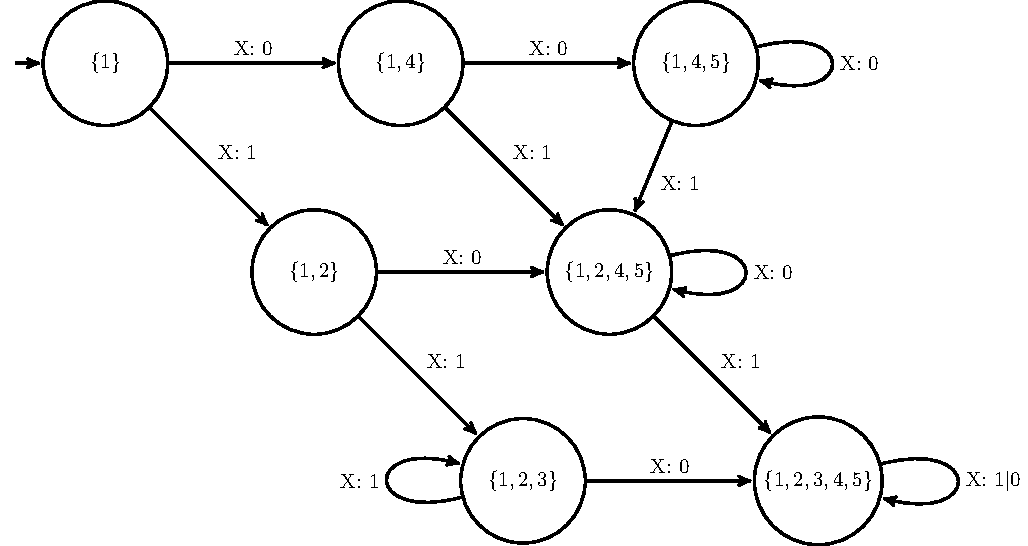
\includegraphics{antichain-meets-projection.pdf}}
 \end{center}
\end{figure}
	\end{frame}
	
	\section{Srovnání přístupů}
	\begin{frame}{Srovnání z hlediska času}
	\only<1>{
	\begin{itemize}
	\item Srovnání na rodině formulí:
	$$\varphi_n \overset{\mathit{def}}{=} \exists X\forall x_1\ldots x_n.
 \bigwedge_{i = 1}^{n-1} (x_i \in X \Rightarrow x_{i+1} \in X)$$
\end{itemize}}
  \only<2>{
	\begin{center}
		\scalebox{0.8}{\input{fig/szz2.tex}}
	\end{center}}
	\end{frame}
	
	\begin{frame}{Srovnání generovaného prostoru}
	\begin{center}
	\scalebox{0.8}{\input{fig/szz1.tex}}
	\end{center}
	\end{frame}
	
	\begin{frame}{Závěrečné shrnutí}
	\begin{itemize}
	 \item Představena logika WS$k$S a přístupy k jejímu rozhodování:
	 \begin{enumerate}
	  \item Pomocí DTA $\rightarrow$ \textsc{MONA}
		\item Pomocí NTA $\rightarrow$ \texttt{dWiNA}
	 \end{enumerate}
	\pause
	\smallskip
	 \item Nástroje srovnány z hlediska rychlosti a generovaného prostoru
	\smallskip
	\pause
	 \item Výsledky:
	 \begin{itemize}
	  \item Pro jistou třídu formulí:
		 \begin{itemize}
		  \item Řádově rychlejší rozhodování než nástrojem \textsc{MONA}
			\item Znatelná redukce prohledávaného stavového prostoru
		 \end{itemize}
		\item 3. místo na studentské konferenci EEICT
	 \end{itemize}
	\smallskip
	\pause
	\item Výhledy do budoucna?
	 \begin{itemize}
	  \item[$\Rightarrow$] Rozšíření a publikace na zahraniční konferenci!
	 \end{itemize}
	\end{itemize}
	\end{frame}
	
% All your regular slides
% After your last numbered slide
\appendix
\newcounter{finalframe}
\setcounter{finalframe}{\value{framenumber}}

	\begin{frame}{Otázky oponenta}
	\begin{block}{1. Co by bylo nutné udělat pro kompilaci dWiNA pomocí 64bit. kompilátorů?}
	\begin{center}
	\begin{enumerate}
	 \item Závislost na knihovně \texttt{libvata}
	\pause
	 \begin{itemize}
	  \item[$\Rightarrow$] Řešení = přilinkování 64bit knihovny
	 \end{itemize}
	\pause
	 \item Závislost na několika knihovnách nástroje \texttt{MONA}
	\pause
	 	 \begin{itemize}
	  \item[$\Rightarrow$] Řešení = odstranit tuto závislost
	 \end{itemize}
	\pause
	\item Parametrický překlad podle architektury pomocí nástroje \texttt{cmake}
	\pause
	\end{enumerate}
	\end{center}
	\end{block}
	\end{frame}

% Backup frames
\setcounter{framenumber}{\value{finalframe}}
\end{document}
